\documentclass{article}
\usepackage{graphicx} % Required for inserting images
\usepackage[italian]{babel}
\usepackage{amsmath}
\usepackage[hidelinks]{hyperref}
\usepackage{float}
\usepackage{multicol}

\newcommand{\df}{\noindent\textbf{Definizione }}

\title{Organizzazione e gestione per lo start-up aziendale}
\author{Leonardo Ganzaroli}
\date{}

\begin{document}

\maketitle

\addcontentsline{toc}{section}{\protect\numberline{}Introduzione}

\tableofcontents

\newpage

\hypersetup{allcolors=black}

\section*{Introduzione}

Questi appunti sono derivanti principalmente dalle dispense del corso di \textit{Organizzazione e gestione per lo start-up aziendale} che ho seguito durante la laurea Triennale di informatica all'università "La Sapienza".

\newpage

\section{Bisogni}

\df Un'organizzazione è uno strumento utilizzato dalle persone per coordinare le loro azioni ed ottenere valore.\newline

\df L'imprenditorialità è il processo con il quale le persone riconoscono le opportunità per soddisfare i bisogni, andando poi ad ottenere ed usare le risorse necessarie a quel processo.\newline

\df I bisogni sono una sensazione di insoddisfazione psico-fisica accompagnata dalla consapevolezza dell’esistenza di un bene atto a rimuovere o ad attenuare la sensazione stessa, si distinguono:
\begin{enumerate}
    \item \textbf{Fisici}, legati alla sopravvivenza fisica di un essere umano.
    \item \textbf{Psichici/Spirituali}, collegati allo stato psichico di un essere umano.
\end{enumerate}

\noindent Si possono classificare in base a:
\begin{itemize}
    \item \textbf{Risorgenza}
        \begin{itemize}
            \item Continui
            \item Periodici
            \item Eccezionali
        \end{itemize}
    \item \textbf{Soggettività}

        Possono variare nel tempo e nello spazio.
    
    \item \textbf{Priorità}
        \begin{itemize}
            \item Rigidi
            \item Elastici\newline
        \end{itemize}
\end{itemize}

\noindent L'attività effettiva per soddisfare questi bisogni si può dividere in 2 fasi:

\begin{figure}[ht]
    \centering
    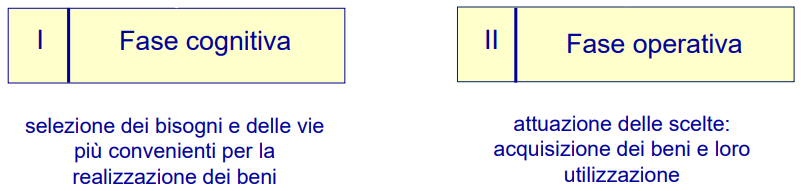
\includegraphics[width=0.9\linewidth]{bis.png}
\end{figure}

\newpage

\noindent Più nello specifico:

\begin{figure}[H]
    \centering
    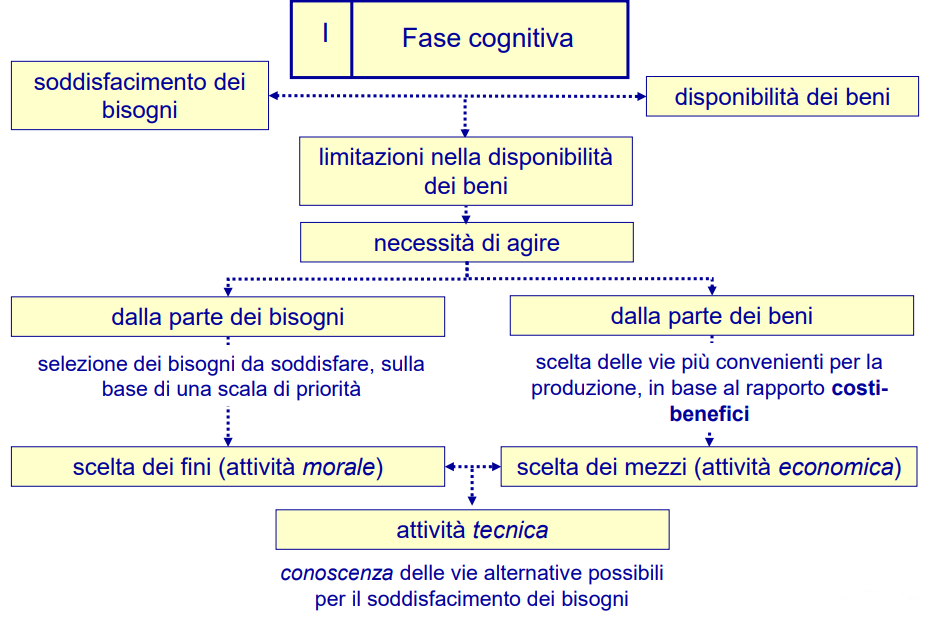
\includegraphics[width=\linewidth]{f1.png}
    \noindent\rule{\textwidth}{0.5pt}\newline
\end{figure}

\begin{figure}[H]
    \centering
    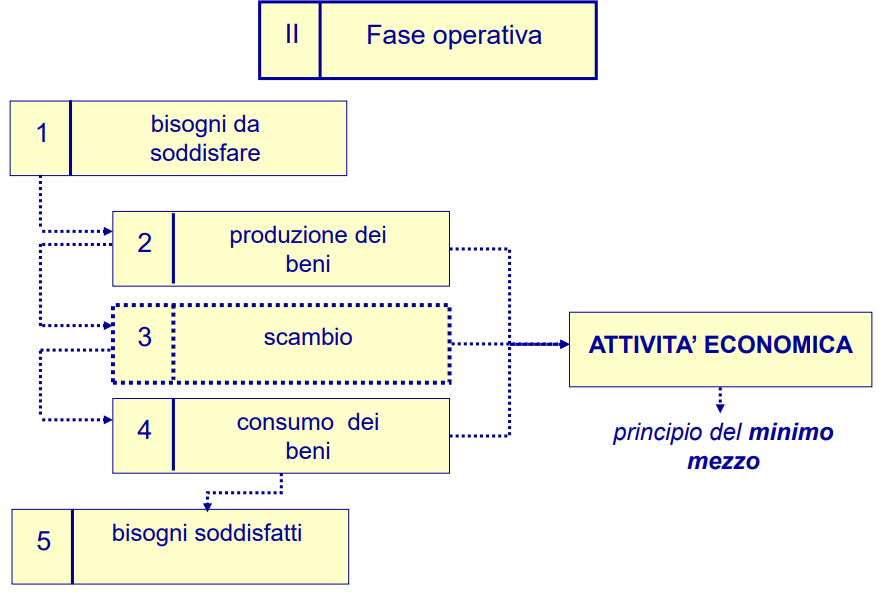
\includegraphics[width=0.9\linewidth]{f2.png}
\end{figure}

\newpage

\noindent La stessa produzione è formata da più tipi di trasformazione del bene:\newline

\begin{figure}[ht]
    \centering
    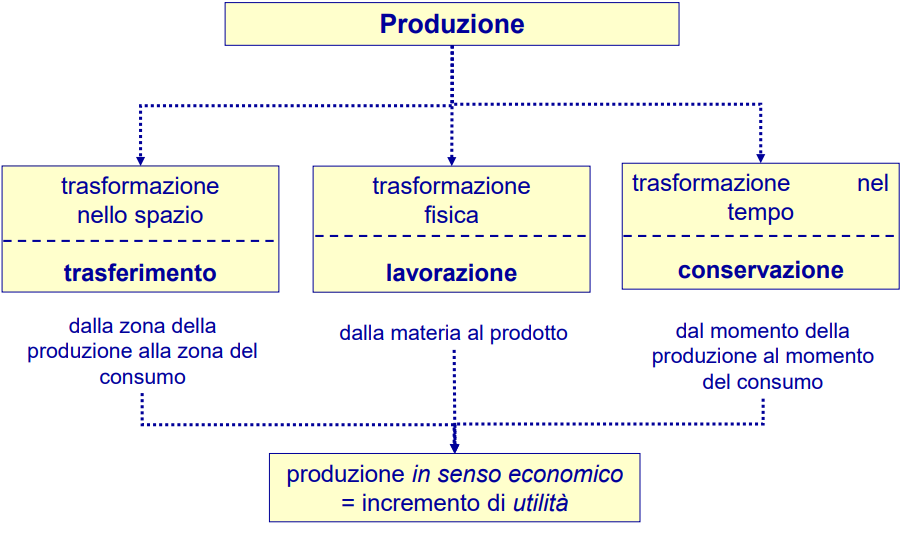
\includegraphics[width=\linewidth]{prod.png}
\end{figure}

\noindent Tutto il processo visto si può riassumere in produzione e consumo dei beni, ogni atto compreso in esso viene svolto dai \textit{Gruppi economici}. Questi hanno subito un'evoluzione nel corso nel tempo, i 3 step principali sono stati:
\begin{enumerate}
    \item \textbf{Fase autarchica}

        Il gruppo si occupa di tutta la produzione necessaria per il proprio consumo.

    \item \textbf{Specializzazione}

        Un gruppo si dedica solamente ad alcune produzioni ed ottiene le altre tramite scambi.

    \item \textbf{Diversificazione}

        Si verifica una scissione del gruppo in:
            \begin{itemize}
                \item Gruppo di produzione
                \item Gruppo di consumo\newline
            \end{itemize}    
\end{enumerate}

\noindent Quest'ultimo permette di dividere il processo di soddisfacimento in:
    \begin{itemize}
        \item \textbf{Indiretto}

            La produzione effettuata dalle aziende.
        
        \item \textbf{Diretto}

            Il consumo effettuato dalle famiglie.
        
    \end{itemize}

\section{L'azienda}

\df L'azienda si può definire in diversi modi:
\begin{itemize}
    \item Un istituto economico atto a perdurare
    \item Lo strumento dell’operare umano in campo economico
    \item Un sistema di elementi orientato al raggiungimento di un fine
    \item L’unità economica elementare per il conseguimento degli scopi economici degli esseri umani
    \item Una coordinazione economica in atto che stabilisce rapporti biunivoci con l’ambiente in cui opera
    \item La forma organizzativa della produzione tipica della società moderna, inserita in un più ampio contesto economico e sociale\newline
\end{itemize}

\noindent Si distinguono:
\begin{itemize}
    \item In base al numero di individui che la compongono
        \begin{itemize}
            \item Azienda \textbf{individuale}
            \item Azienda \textbf{collettiva}
        \end{itemize}
    \item In base alla sua natura
        \begin{itemize}
            \item Azienda \textbf{privata}
            \item Azienda \textbf{pubblica}\newline
        \end{itemize}
\end{itemize}

\noindent Un tipo particolare di aziende sono quelle finanziarie, esse si occupano della fornitura dei mezzi finanziari necessari alla produzione ed il consumo.\newline

\noindent Un'ulteriore distinzione è data dalla finalità di un'azienda:
\begin{itemize}
    \item Scopo di \textbf{lucro}
        \begin{itemize}
            \item Imprese
        \end{itemize}
    \item Scopo \textbf{non di lucro}
        \begin{itemize}
            \item Associazioni
            \item Fondazioni
            \item Enti politico-sociali
            \item $\ldots$
        \end{itemize}
\end{itemize}

\newpage

\df Il sistema economico generale è dato dalle relazioni tra aziende e famiglie, nello specifico:

\begin{figure}[ht]
    \centering
    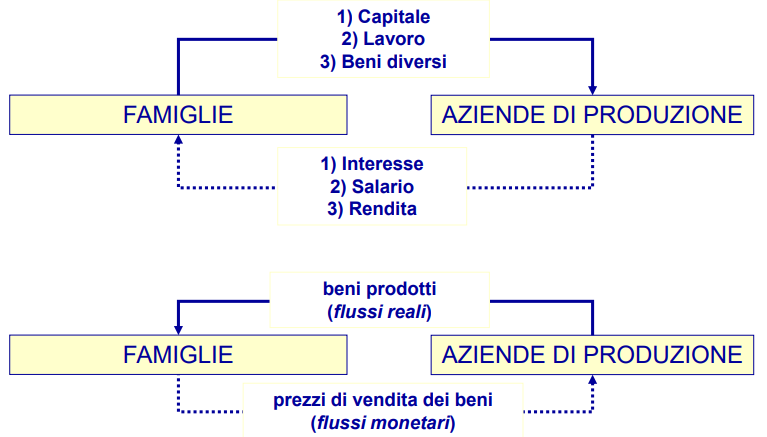
\includegraphics[width=0.95\linewidth]{rel.png}
\end{figure}

\subsection{Elementi costitutivi}

\begin{figure}[ht]
    \centering
    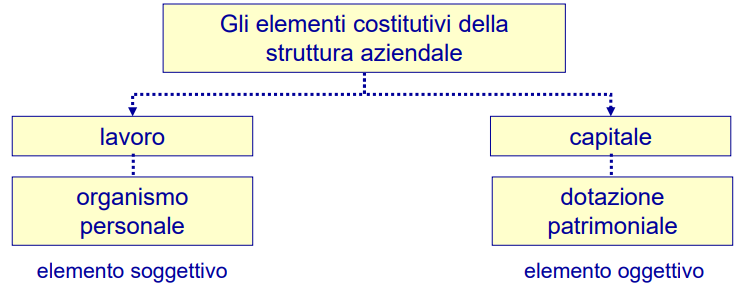
\includegraphics[width=0.9\linewidth]{st_az.png}
\end{figure}

\noindent L'impegno umano coinvolto in un'azienda si può dividere in:
\begin{itemize}
    \item \textbf{Volitivo}

        Il concepimento delle linee guida generali di svolgimento dell’attività.

    \item \textbf{Direttivo}

        Il concepimento delle linee guida specifiche di svolgimento dell'attività.
    
    \item \textbf{Esecutivo}

        L'attuazione delle linee guida del punto precedente.\newline
    
\end{itemize}

\noindent Essi fanno parte delle varie fasi della vita aziendale:
\begin{enumerate}
    \item Progettazione dell'azienda
        \begin{itemize}
            \item Creazione del disegno
            \item Composizione delle linee fondamentali
        \end{itemize}
    \item Inserimento del capitale monetario
    \item Acquisizione dei fattori produttivi

        \vspace{5pt}

        Il capitale passa da generico a specifico.\newline

        I fattori sono:
        \begin{itemize}
            \item Utilità materiali e non
            \item Lavoro direttivo ed esecutivo\newline
        \end{itemize}
\end{enumerate}

\noindent In sintesi:

\begin{figure}[ht]
    \centering
    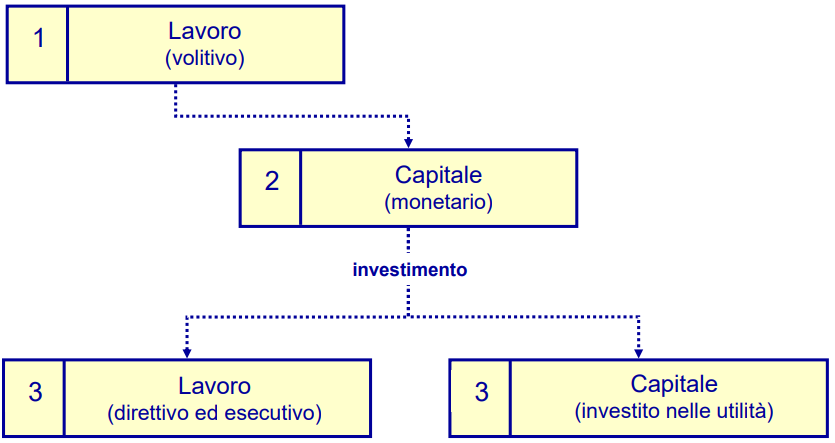
\includegraphics[width=0.9\linewidth]{fasi.png}
\end{figure}

\newpage

\subsection{Gestione}

\df La gestione è il complesso delle azioni che le persone svolgono sul capitale, consiste di:\newline

\begin{figure}[ht]
    \centering
    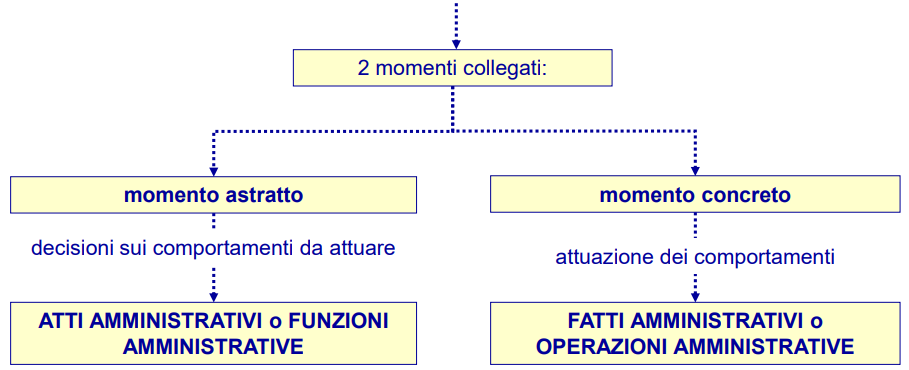
\includegraphics[width=\linewidth]{gest.png}
\end{figure}

\noindent Il lavoro va quindi ad agire sul capitale prima tramite decisioni e poi tramite le operazioni che ne conseguono, queste possono avere degli effetti:
\begin{itemize}
    \item \textbf{Qualitativi}, modificano la composizione    
    \item \textbf{Quantitativi}, modificano la dimensione\newline
\end{itemize}

\noindent Il percorso che porta dalle prime alle seconde si riassume come:

\begin{figure}[ht]
    \centering
    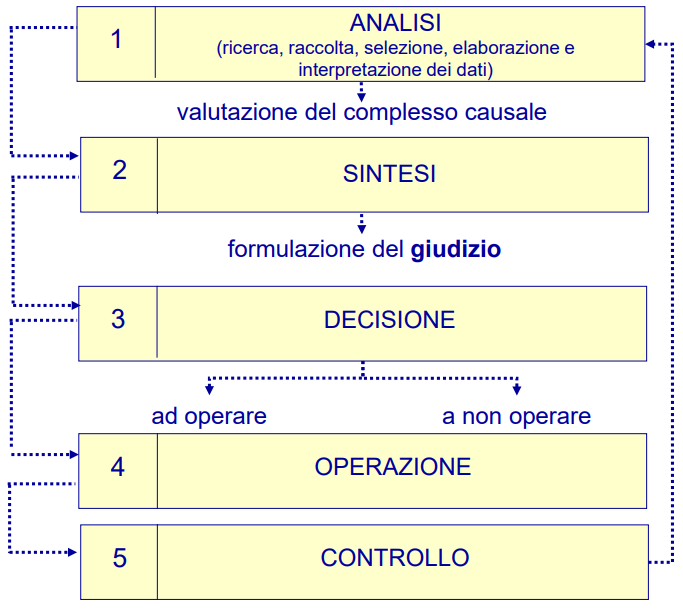
\includegraphics[width=0.7\linewidth]{funz_op.png}
\end{figure}

\noindent Durante le varie fasi di vita si distinguono diverse funzioni:
\begin{itemize}
    \item \textbf{Istituzionali}
    \item \textbf{Di funzionamento}
    \item \textbf{Terminali}\newline
\end{itemize}

\df Il collegamento e l'interdipendenza tra le funzioni dà origine ad un sistema delle funzioni che a loro volta danno origine ai processi o a combinazioni di processi.\newline

\noindent Le decisioni portano ad una condizione di incertezza dato che non si conoscono gli eventuali effetti scaturiti da esse, la gestione stessa si svolge sempre in un clima di incertezza.\newline

\begin{figure}[ht]
    \centering
    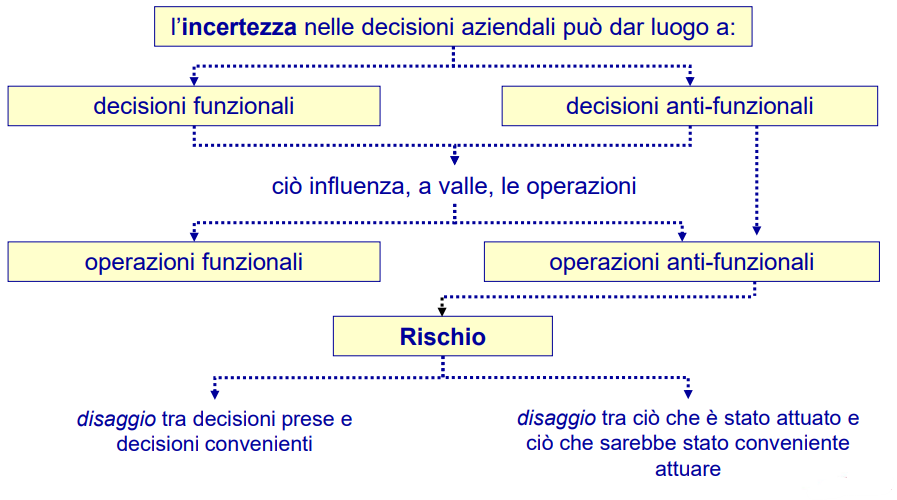
\includegraphics[width=\linewidth]{inc.png}
\end{figure}

\subsection{Figure amministrative}

\begin{itemize}
    \item \textbf{Nell'azienda individuale}

    \vspace{5pt}

    \df Il titolare/imprenditore svolge diversi ruoli:
        \begin{itemize}
            \item Concentra sulla sua persona la titolarità dei diritti e delle obbligazioni
            \item Sopporta il rischio
            \item Presta lavoro volitivo e direttivo
            \item Apporta il capitale
            \item Esercita potere decisionale
        \end{itemize}

    2 definizioni vengono date nel codice civile:
        \begin{itemize}
            \item \href{https://www.gazzettaufficiale.it/atto/serie_generale/caricaArticolo?art.versione=1&art.idGruppo=262&art.flagTipoArticolo=2&art.codiceRedazionale=042U0262&art.idArticolo=2082&art.idSottoArticolo=1&art.idSottoArticolo1=10&art.dataPubblicazioneGazzetta=1942-04-04&art.progressivo=0}{Art. 2082}
            \item \href{https://www.gazzettaufficiale.it/atto/serie_generale/caricaArticolo?art.versione=2&art.idGruppo=262&art.flagTipoArticolo=2&art.codiceRedazionale=042U0262&art.idArticolo=2086&art.idSottoArticolo=1&art.idSottoArticolo1=10&art.dataPubblicazioneGazzetta=1942-04-04&art.progressivo=0}{Art. 2086}\newline
        \end{itemize}

    In un'azienda indivduale esso è sia soggetto giuridico che economico.

    \begin{figure}[ht]
        \centering
        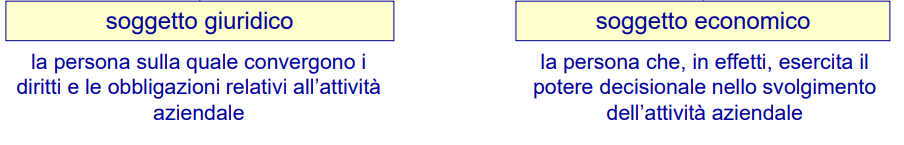
\includegraphics[width=\linewidth]{sogg.png}
    \end{figure}

    Può però delegare il potere decisionale ad un amministratore/direttore che diventa soggetto economico.\newline

    Gli impegni di un imprenditore sono quindi:\newline
    
    \begin{figure}[ht]
    \centering
    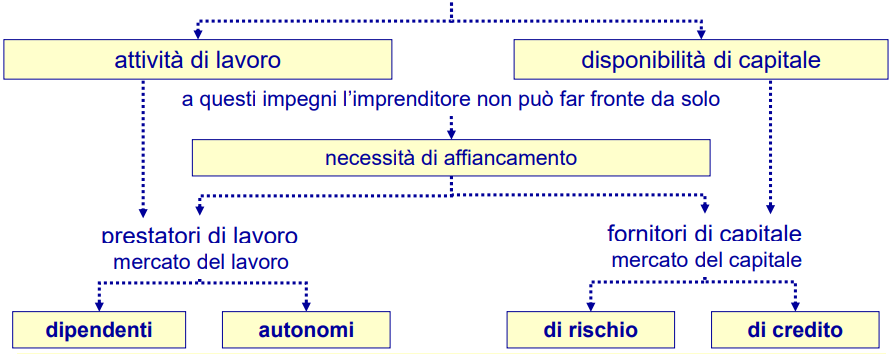
\includegraphics[width=\linewidth]{impr.png}
    \end{figure}

    Alcuni articoli utili (sempre cod. civ.):
        \begin{itemize}
            \item \href{https://www.gazzettaufficiale.it/atto/serie_generale/caricaArticolo?art.versione=2&art.idGruppo=263&art.flagTipoArticolo=2&art.codiceRedazionale=042U0262&art.idArticolo=2094&art.idSottoArticolo=1&art.idSottoArticolo1=10&art.dataPubblicazioneGazzetta=1942-04-04&art.progressivo=0}{2094}
            \item \href{https://www.gazzettaufficiale.it/atto/serie_generale/caricaArticolo?art.progressivo=0&art.idArticolo=2095&art.versione=2&art.codiceRedazionale=042U0262&art.dataPubblicazioneGazzetta=1942-04-04&art.idGruppo=263&art.idSottoArticolo1=10&art.idSottoArticolo=1&art.flagTipoArticolo=2}{2095}
            \item \href{https://www.gazzettaufficiale.it/atto/serie_generale/caricaArticolo?art.versione=1&art.idGruppo=283&art.flagTipoArticolo=2&art.codiceRedazionale=042U0262&art.idArticolo=2222&art.idSottoArticolo=1&art.idSottoArticolo1=10&art.dataPubblicazioneGazzetta=1942-04-04&art.progressivo=0}{2222}\newline
        \end{itemize}
    
    \item \textbf{Nelle società}

        In questo caso è presente una divisione:
            \begin{itemize}
                \item Il soggetto economico è il consiglio di amministrazione o l'amministratore delegato
                \item Il soggetto giuridico è la società stessa
                \item Il rischio resta ai soci (in base alle azioni sottoscritte)
            \end{itemize}
    
\end{itemize}

\subsection{Equilibrio economico}

Usando un altro punto di vista si può ridefinire l'azienda:\newline

\begin{figure}[ht]
    \centering
    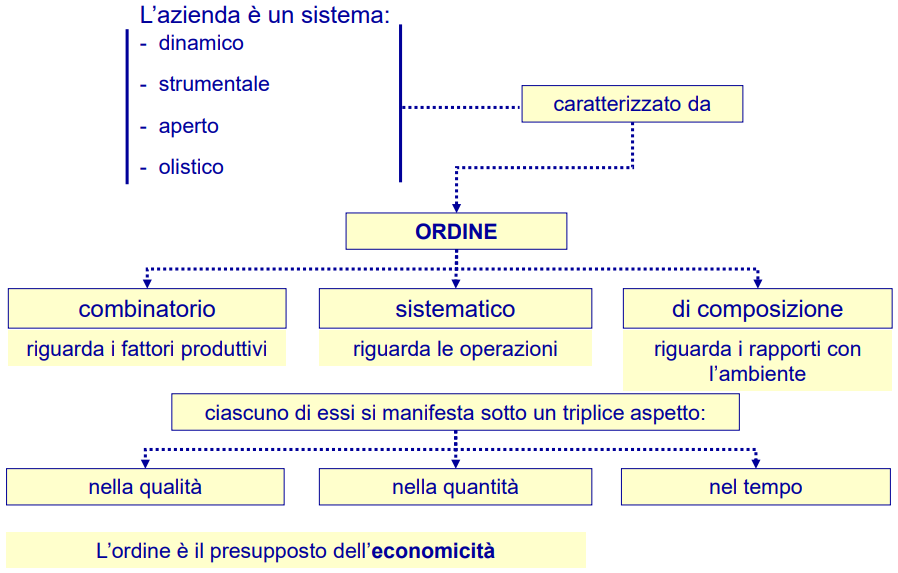
\includegraphics[width=\linewidth]{sist.png}
\end{figure}

\noindent Tutto il processo di gestione si può vedere come un insieme di flussi di energia:
\begin{itemize}
    \item \textbf{Cessione}, acquisizione ed uso dei fattori (Costi)
    \item \textbf{Reintegro}, vendita del prodotto ottenuto (Ricavi)\newline
\end{itemize}

\noindent L'equilibrio economico si verifica quando $\text{Ricavi}\geq\text{Costi}$, in alcuni casi i costi figurativi (interesse partimoniale, permio-rischio, remunerazione direzionale) non vengono considerati nei fattori e vanno sommati ai costi ($\text{Costi}+M$).\newline

\noindent Inoltre è necessario che i ricavi coprano (oltre ai costi storici) il \textit{deficit} dato dalla differenza tra i costi storici e le prospettive dei costi per l'acquisto dei nuovi fattori.\newline

\df L'economicità è la capacità di mantenersi in equilibrio economico.\newline

\df La redditività è la capacità di generare redditi positivi.

\newpage

\section{L'ambiente}

\df L'ambiente esterno è costituito dall’insieme degli attori e delle forze esterne all’impresa che ne influenzano la performance.\newline

\begin{figure}[ht]
    \centering
    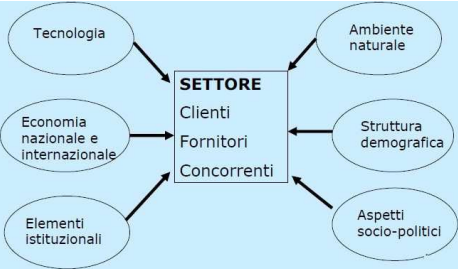
\includegraphics[width=0.65\linewidth]{amb.png}
    \caption{Schema ambiente}
\end{figure}

\noindent Per avere una visione più approfondita l'ambiente viene diviso in settori:

\begin{figure}[ht]
    \centering
    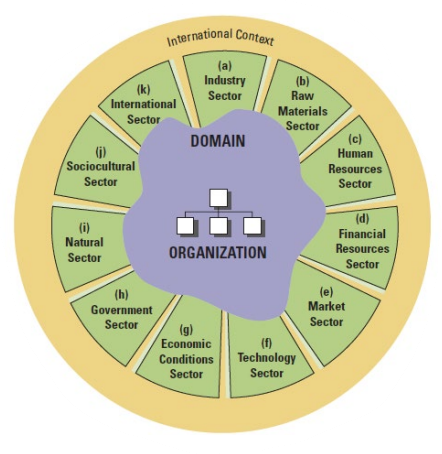
\includegraphics[width=0.6\linewidth]{amb2.png}
\end{figure}

\noindent Per descrivere gli eventi e i modelli dell'ambiente si individuano:
\begin{itemize}
    \item Dinamismo
    \item Complessità
    \item Abbondanza (di risorse finanziarie)
\end{itemize}

\noindent I vari valori assunti sono correlati ai diversi gradi di incertezza che possono presentarsi:

\begin{table}[ht]
    \centering
    \begin{tabular}{c|c|c}
        Dinamismo$\setminus$Complessità & Bassa & Alta\\
         \hline
        Basso & Bassa & Medio-bassa\\
        \hline
        Alto & Medio-alta & Alta\\
    \end{tabular}
    \caption{Gradi di incertezza}
\end{table}

\noindent Per cercare di adattarsi all'ambiente bisogna adattare la struttura interna, ci sono diversi metodi:
\begin{itemize}
    \item Aggiungere posizioni e/o dipartimenti
    \item Costruire relazioni
    \item Differenziare/Integrare i dipartimenti\newline
\end{itemize}

\noindent Un altro fattore importante è quanta dipendenza ci sia dalle altre organizzazioni, se la maggior parte delle risorse sono controllate da altri si presenta un problema di vulnerabilità. Per ovviare al problema bisogna cercare di controllare gli elementi dell'ambiente:
\begin{itemize}
    \item Stabilire relazioni formali
        \begin{itemize}
            \item Acquisire una quota di proprietà
            \item Formare joint venture
            \item Fare interlocking
            \item Reclutare dirigenti
            \item Usare PR e pubblicità
        \end{itemize}
    \item Influenzare settori chiave
        \begin{itemize}
            \item Cambiare luogo di attività
            \item Lobbying
            \item Partecipare alle associazioni di categoria
            \item Attività illegittime
        \end{itemize}
\end{itemize}

\newpage

\subsection{Porter}

\noindent Un modello usato per rappresentare l'ambiente e conseguentemente valutare la posizione competitiva di un'azienda è quello di Porter, esso identifica 5 attori principali con le rispettive forze:

\begin{figure}[ht]
    \centering
    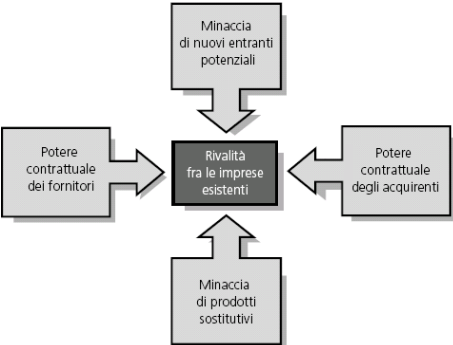
\includegraphics[width=0.55\linewidth]{porter.png}
    \caption{Modello di Porter}
\end{figure}

\vspace{5pt}

\begin{figure}[ht]
    \centering
    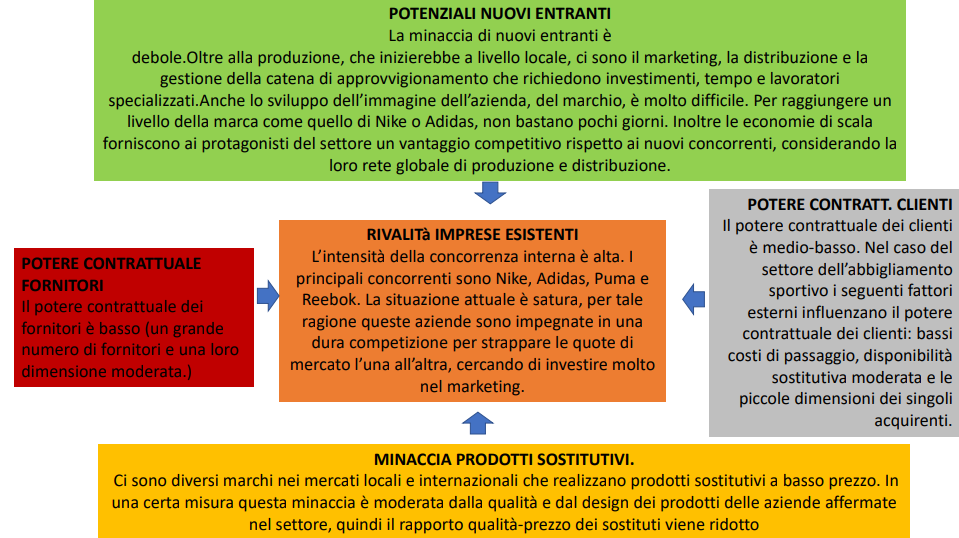
\includegraphics[width=\linewidth]{porter2.png}
    \caption{Esempio abbigliamento sportivo}
\end{figure}

\newpage

\subsection{Burns \& Stalker, Chandler}

Il modello di Burns \& Stalker dimostra che l'\hyperref[fig:assetto]{assetto organizzativo} viene influenzato dal tipo di ambiente ed il contesto in cui si trova.\newline

\begin{figure}[ht]
    \centering
    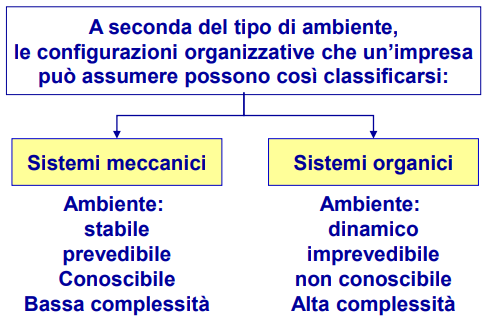
\includegraphics[width=0.65\linewidth]{bs.png}
\end{figure}

\noindent In particolare:
\begin{itemize}
    \item La struttura organizzativa dipende da:
        \begin{itemize}
            \item Formalizzazione
            \item Standardizzazione
            \item Specializzazione
            \item Centralizzazione
        \end{itemize}
    \item Lo stile di direzione dipende da:
        \begin{itemize}
            \item Modello decisionale
            \item Legittimazione del potere
        \end{itemize}
    \item I meccanismi operativi dipendono da:
        \begin{itemize}
            \item Programmazione e controllo
            \item Comunicazione
            \item Gestione del personale\newline
        \end{itemize}
\end{itemize}

\noindent Il rapporto tra strategia e struttura (Chandler, 1969) dimostra, in chiave storica, come durante le diverse fasi del capitalismo e dello sviluppo industriale siano emersi dei modelli organizzativi sempre più complessi e sofisticati.

\section{L'organizzazione}

L'oggetto dell'organizzazione è il lavoro, le decisioni organizzative riguardano:
\begin{itemize}
    \item Divisione del lavoro tra gli operatori
    \item Meccanismi di coordinamento
    \item Autonomia decisionale degli operatori
    \item Flussi di informazione e decisione
    \item Rapporto tra contributi ed incentivi\newline
\end{itemize}

\begin{figure}[ht]
    \centering
    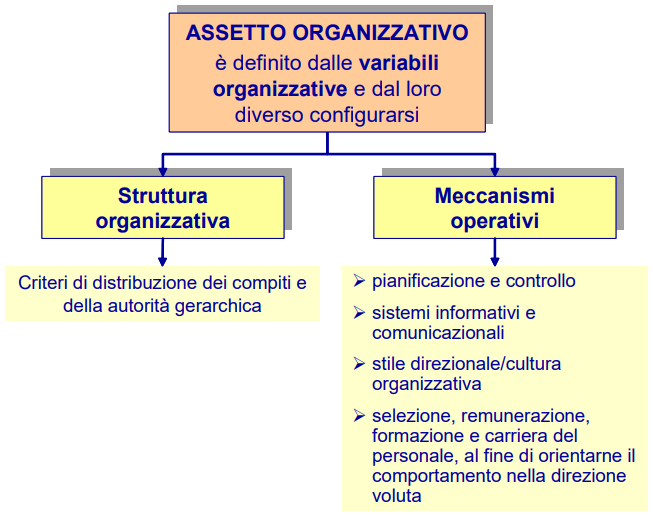
\includegraphics[width=0.8\linewidth]{org.png}
    \label{fig:assetto}
\end{figure}

\vspace{5pt}

\noindent Il processo di creazione dell'assetto richiede che vengano esplicitati:
\begin{itemize}
    \item Gli attori rilevanti
    \item Gli obiettivi che si vogliono raggiungere
    \item Il ruolo della struttura nel futuro
\end{itemize}

\newpage

\subsection{Struttura organizzativa}

\df L'organigramma rappresenta visivamente un insieme di attività e processi sottostanti ad un'organizzazione.\newline

\noindent I tipi di collegamenti presenti identificano la condivisione delle informazioni:
\begin{itemize}
    \item \textbf{Verticali}

        Progettati per il controllo.
    
    \item \textbf{Orizzontali}

        Progettati per il coordinamento e la collaborazione.
    
\end{itemize}
\noindent Le strutture principalmente verticali presentano una divisione a livelli gerarchici, questo comporta un sistema decisionale centralizzato.\newline

\noindent Per inserire collegamenti orizzontali si possono usare:
\begin{itemize}
    \item Sistemi informativi
    \item Ruoli di collegamento
    \item Task force
    \item Integratori a tempo pieno
    \item Team interfunzionali\newline
\end{itemize}

\noindent I possibili raggruppamenti per dipartimento sono:
\begin{itemize}
    \item \textbf{Funzionale}
    
        Quello classico.
    \item \textbf{Divisionale}

        Come il precedente ma presenta una divisione per prodotti.
    
    \item \textbf{A matrice}

        Una fusione dei precedenti.
    
    \item \textbf{A rete virtuale}

        Sub-appalti di funzioni ad esterni.
    
    \item \textbf{Olocrazia}

        Spostamento all'autogestione.
    
\end{itemize}

\newpage

\noindent Rispettivi organigrammi:

\begin{figure}[ht]
    \centering
    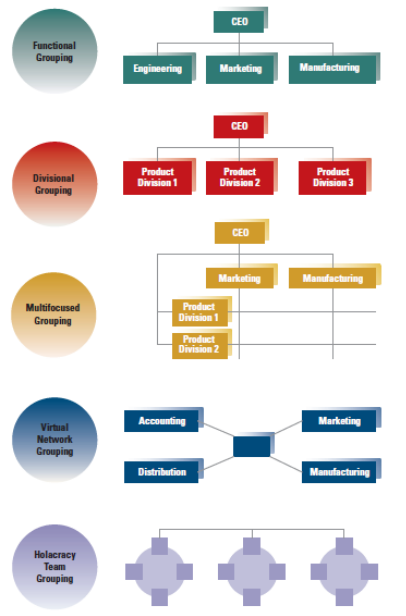
\includegraphics[width=0.6\linewidth]{orga.png}
\end{figure}

\newpage

\subsection{Approccio Razionale-Centralizzato}

\begin{figure}[ht]
    \centering
    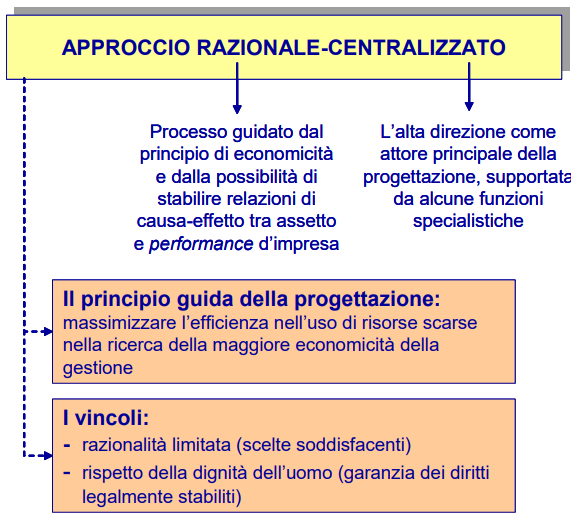
\includegraphics[width=0.7\linewidth]{arc.png}
\end{figure}

\vspace{5pt}

\noindent Il paradigma di appartenenza di questo approccio asserisce che:
\begin{itemize}
    \item L'efficienza dell'impresa è funzione delle combinazioni tra la configurazione ambientale e quella organizzativa
    \item In condizioni di efficienza le due configurazioni sono correlate
    \item Non esiste una corrispondenza biunivoca tra tipo di ambiente e tipo di assetto, il rapporto tra i 2 è mediato dalla strategia\newline
\end{itemize}

\noindent Le caratteristiche dell'assetto dipendono quindi da:
\begin{itemize}
    \item L'ambiente operativo
    \item Gli orientamenti strategici
    \item Le tecnologie usate
    \item Le caratteristiche del personale
\end{itemize}

\newpage

\subsection{Equilibrio ed efficienza}

\begin{figure}[ht]
    \centering
    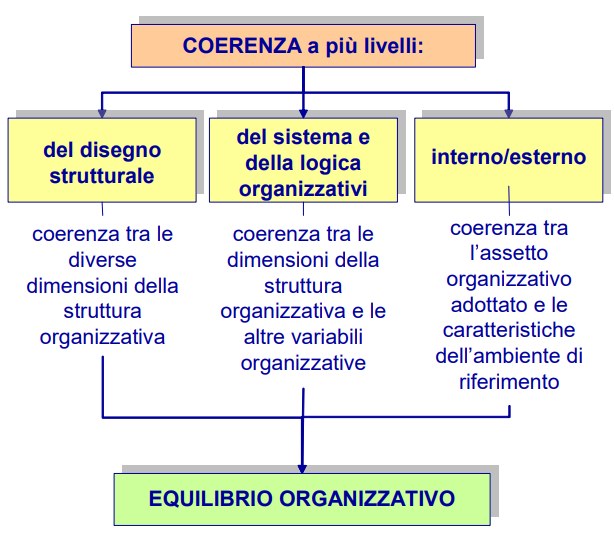
\includegraphics[width=0.7\linewidth]{coer.png}
\end{figure}

\vspace{4pt}

\noindent Per valutare i risultati di un certo comportamento organizzativo bisogna considerare gli obiettivi voluti:

\begin{figure}[ht]
    \centering
    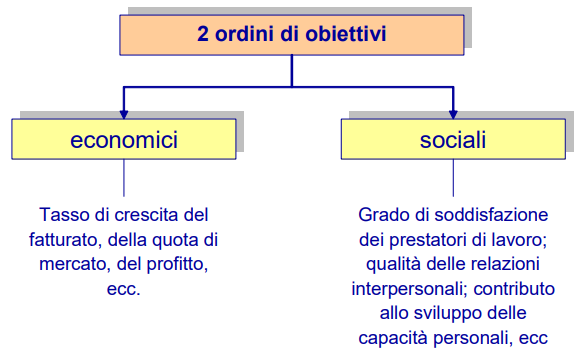
\includegraphics[width=0.7\linewidth]{ob.png}
\end{figure}

\df L'efficacia è il grado di raggiungimento degli obiettivi.\newline

\df L'efficienza è il costo sostenuto per raggiungere un certo grado di efficacia.\newline

\df L'economicità duratura è la capacità di soddisfare interessi istituzionali.

\newpage

\subsection{Microstruttura}

\begin{figure}[ht]
    \centering
    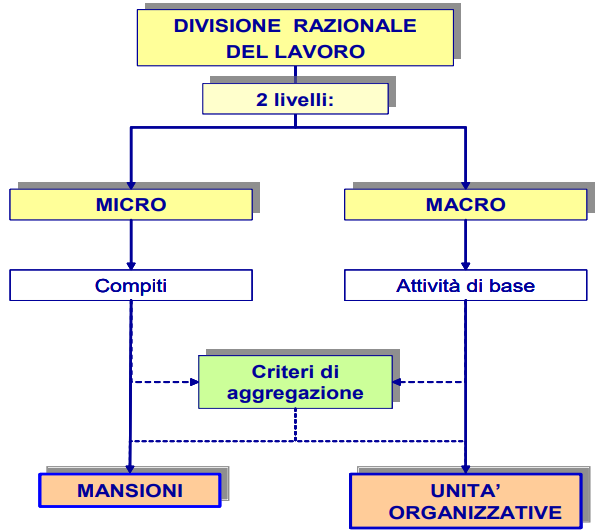
\includegraphics[width=0.7\linewidth]{micro.png}
\end{figure}

\vspace{4pt}

\df Un compito è un insieme di attività affidate ad un individuo, può essere:
\begin{itemize}
    \item \textbf{Formalizzabile}

        Si possono esplicitare regole/norme/procedure per svolgerlo.

    \item \textbf{Standardizzabile}

        Si può rendere ripetibile sempre nello stesso modo.\newline
    
\end{itemize}

\df Una mansione è un insieme di compiti, ha le seguenti caratteristiche:
\begin{itemize}
    \item Grado di varietà
    \item Grado di autonomia
    \item Grado di contribuzione
    \item Grado di interazione sociale
\end{itemize}

\noindent Agli estremi si individuano le mansioni ricche e quelle povere, le seconde possono essere migliorate con una riprogettazione:
\begin{itemize}
    \item \textbf{Rotazione}
    \item \textbf{Allargamento}
    \item \textbf{Arricchimento}
\end{itemize}

\subsection{Zero-base Review}

Questo modello permette di aggregare le attività di base secondo certe logiche cercando di massimizzare l'efficienza, risulta utile anche per trovare delle soluzioni in caso di emersione di sintomi disfunzionali nell'organizzazione.\newline

\noindent Obiettivi:
\begin{itemize}
    \item Minimizzare i costi di coordinamento e controllo
    \item Massimizzare economie di scala/specializzazione\newline
\end{itemize}

\noindent Per fare ciò si seguono i seguenti step:
\begin{enumerate}
    \item Mappare le attività di base
    \item Analizzare le interdipendenze, ci sono 3 tipi:
        \begin{enumerate}
            \item Generica $\rightarrow$ Standardizzazione (G)
            \item Sequenziale $\rightarrow$ Pianificazione (S)
            \item Reciproca $\rightarrow$ Mutuo aggiustamento (R)

                A parità di altre condizioni quest'ultime vengono assegnate alla stessa unità.
            
        \end{enumerate}
    \item Analizzare le affinità tecniche (T)
    \item Analizzare le affinità di orientamento (O)    
    \item Definire dei \textit{cluster} di attività
    \item Controllare le nuove dimensioni\newline
\end{enumerate}

\noindent\rule{\textwidth}{0.5pt}\newline
Esempio:

\begin{table}[ht]
    \centering
    \begin{tabular}{c|c|c|c|c|c|c|c|c}
        Attività & 1 & 2 & 3 & 4 & 5 & 6 & 7 & 8\\
         \hline
        1 & - & R/T/O & S/O & R & G & G & G & G \\
         \hline
        2 & - & - & R/T/O & G & G & G & G & G \\
         \hline
        3 & - & - & - & S-R/T/O & G & G & G & G \\
         \hline
        4 & - & - & - & - & S/T & G & G/O & G/O \\
         \hline
        5 & - & - & - & - & - & S & S/T/O & G/T/O \\
         \hline
        6 & - & - & - & - & - & - & G & G \\
         \hline
        7 & - & - & - & - & - & - & - & S/O \\
         \hline
        8 & - & - & - & - & - & - & - & - \\
    \end{tabular}
\end{table}

\noindent In questo caso 2 cluster potrebbero essere (1,2,3),(4,5,7,8).

\noindent\rule{\textwidth}{0.5pt}\newline

\section{Organizzazioni Digitali e Big Data}

Le organizzazioni tradizionali ("pipe") si possono rappresentare appunto come un tubo in cui entrano le materie prime ed escono i prodotti finiti.\newline

\noindent Con l'evoluzione tecnologica sono nate nuove organizzazioni basate sulle piattaforme, esse non producono beni fisici ma fanno da tramite tra utenti e venditori, si distinguono:
\begin{itemize}
    \item Piattaforme di scambio, interazioni 1:1 (BlaBlaCar)
    \item Piattaforme dei maker, interazioni 1:tanti (Youtube)\newline
\end{itemize}

\noindent Nonostante le ovvie differenze hanno comunque bisogno di una gerarchia e delle regole anche se meno "rigide", per avere un sistema efficace bisogna seguire tre raccomandazioni:
\begin{enumerate}
    \item Avere una cultura costruttiva
    \item Investire nei talenti digitali
    \item Promuovere soft skills e fare team building\newline
\end{enumerate}

\df Per Big Data si intende un qualsiasi insieme di dati di grandi dimensioni, in particolare quelli che superano i limiti tradizionali.\newline

\begin{figure}[ht]
    \centering
    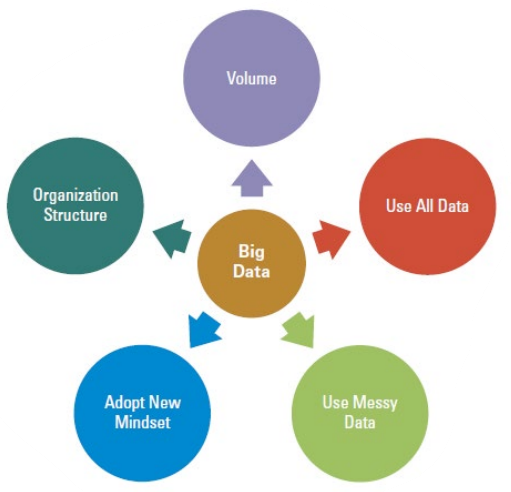
\includegraphics[width=0.55\linewidth]{bigd.png}
    \caption{Elementi di funzionamento}
\end{figure}

\newpage

\noindent L'analisi dei dati è diventata ormai di vitale importanza, un'azienda ha varie scelte per implementarla:
\begin{itemize}
    \item \textbf{Outsourcing}
    \item \textbf{Centralizzato}
    \item \textbf{Design ibrido}
    \item \textbf{Decentralizzato}\newline
\end{itemize}

\begin{figure}[ht]
    \centering
    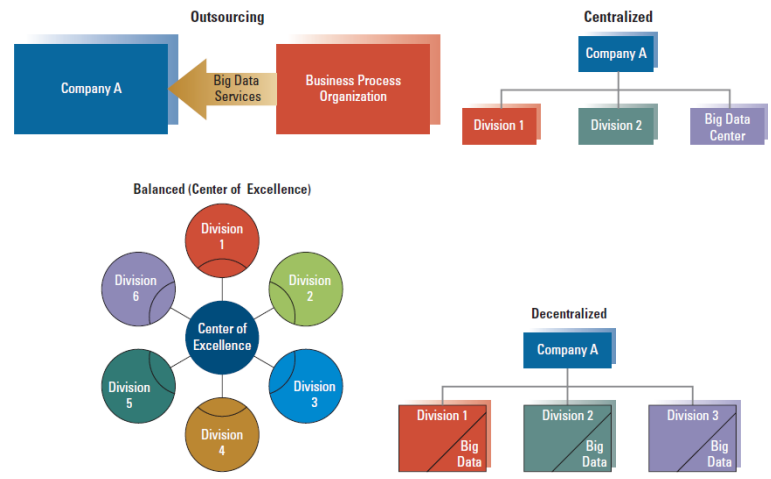
\includegraphics[width=0.9\linewidth]{org_d.png}
    \caption{Rappresentazione visiva}
\end{figure}

\newpage

\section{Relazioni interorganizzative}

\df Le relazioni interorganizzative sono transazioni, flussi e collegamenti tra 2 o più organizzazioni.\newline

\df Un ecosistema organizzativo è un sistema formato dalle interazioni di un insieme di organizzazioni ed il loro ambiente.\newline

\noindent In base al tipo di organizzazioni e relazioni si distinguono:\newline

\begin{table}[ht]
    \centering
    \begin{tabular}{c|c|c}
        Rel.$\setminus$Org. & Diverse & Simili\\
        \hline
        Competitive & Dipendenza dalle risorse & Ecologia della popolazione\\
        \hline
        Cooperative & Reti collaborative & Istituzionalismo\\
    \end{tabular}
\end{table}

\begin{itemize}
    \item \textbf{Dipendenza dalle risorse}

        Le relazioni classiche, si cerca sempre di ridurle al minimo.
    
    \item \textbf{Ecologia della popolazione}

        Basata sulla sopravvivenza, un certo cambiamento può portare alla "morte" di un'organizzazione che non riesce ad adattarsi.
    
    \item \textbf{Reti collaborative}

        Le aziende si "uniscono" per diventare più competitive e condvidere le scarse risorse.
    
    \item \textbf{Istituzionalismo}

        L'obiettivo primario diventa la reputazione nell'ambiente esterno, si cerca quindi di raggiungere l'isomorfismo con le altre organizzazioni. \newline
        
        Per far ciò si usano:
            \begin{itemize}
                \item Forze \textbf{mimetiche}

                    Copiare le aziende di successo.
                
                \item Forze \textbf{coercitive}

                    Adattarsi alle aspettative dell'opinione pubblica o di altri enti.
                
                \item Forze \textbf{normative}

                    Essere sempre in pari con gli standard tecnologici.
                
            \end{itemize}
    
\end{itemize}

\newpage

\section{Altri argomenti}

\subsection{Analisi SWOT}

Quest'analisi permette di definire le possibilità di sviluppo di un sistema aziendale.\newline

\noindent Internamente vanno analizzati i punti di forza e di debolezza, esternamente le opportunità ed eventuali minacce.

\begin{table}[ht]
    \centering
    \begin{tabular}{|c|c|c|}
        \hline
         & Positivo & Negativo\\
         \hline
        Interno & Forze & Debolezze\\
         \hline
        Esterno & Opportunità & Minacce\\
         \hline
    \end{tabular}
\end{table}

\subsection{Balanced scorecard}

La Balanced Scorecard permette di tradurre la missione e le strategie usate in una serie di misure della performance, la struttura generale è la seguente:\newline

\begin{figure}[ht]
    \centering
    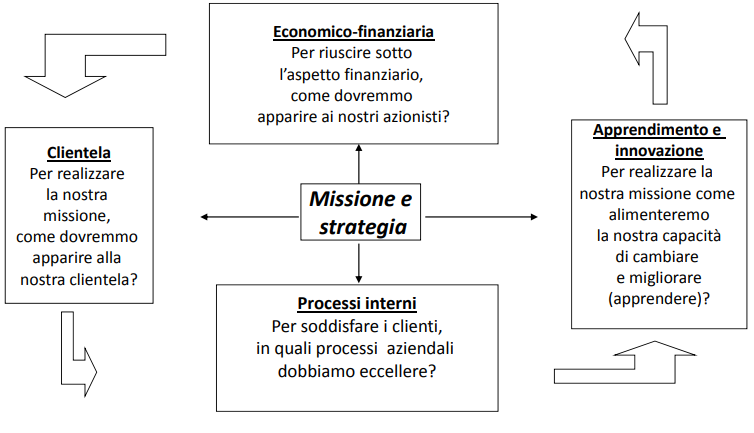
\includegraphics[width=\linewidth]{bsc.png}
\end{figure}

\noindent Per ognuna delle 4 prospettive bisogna considerare:
\begin{multicols}{2}
\begin{itemize}
    \item Obiettivi
    \item Indicatori
    \item Target
    \item Iniziative
\end{itemize}
\end{multicols}

\subsection{Canvas}

Questo modello permette di rappresentare visivamente come un'azienda crea, distribuisce e cattura valore per i clienti, è diviso in 9 sezioni:
\begin{enumerate}
    \item Segmenti di clientela
    \item Proposta di valore
    \item Canali
    \item Relazioni con i clienti
    \item Flussi di ricavi
    \item Risorse chiave
    \item Attività chiave
    \item Partner chiave
    \item Struttura dei costi\newline
\end{enumerate}

\subsection{Indicatori}

\df Il patrimonio netto è una grandezza dello stato patrimoniale ottenuta tramite la differenza tra attività e passività.\newline

\df Il totale attivo di stato patrimoniale è l'insieme di immobilizzazioni e rimanenze di magazzino.\newline

\df Reddito operativo = Margine di guadagno.\newline

\df Il \textit{Return on equity} è la redditività del capitale proprio aziendale, permette di capire quanto un'azienda sia profittevole:
$$\frac{\text{Utile}}{\text{Patrimonio netto}}*100$$\newline

\df Il \textit{Return on investment} è la redditività del capitale investito, analizza quanto gli investimenti fatti possano generare reddito:
$$\frac{\text{Reddito operativo}}{\text{Totale attivo}}*100$$\newline

\end{document}
